\documentclass{article}
\usepackage{graphicx}
\usepackage[margin=1.5cm]{geometry}
\usepackage{amsmath}

\begin{document}

\title{Thursday Reading Assessment: Unit 5, Forces}
\author{Prof. Jordan C. Hanson}

\maketitle

\section{Memory Bank}

\begin{itemize}
\item Stress versus strain relationship: \textit{stress} = Y x \textit{strain}
\item Stress (pressure) is defined like: \textit{stress} = $F/A$, where $F$ is applied force, and $A$ is cross-sectional area.
\item Strain (fractional change in length) is defined like: $\Delta L / L_{0}$, where $L_0$ is the original length of a system, and $\Delta L$ is the change in length.
\item Putting it all together: $F/A = Y (\Delta L/L_{0})$
\end{itemize}
\begin{figure}[ht]
\centering
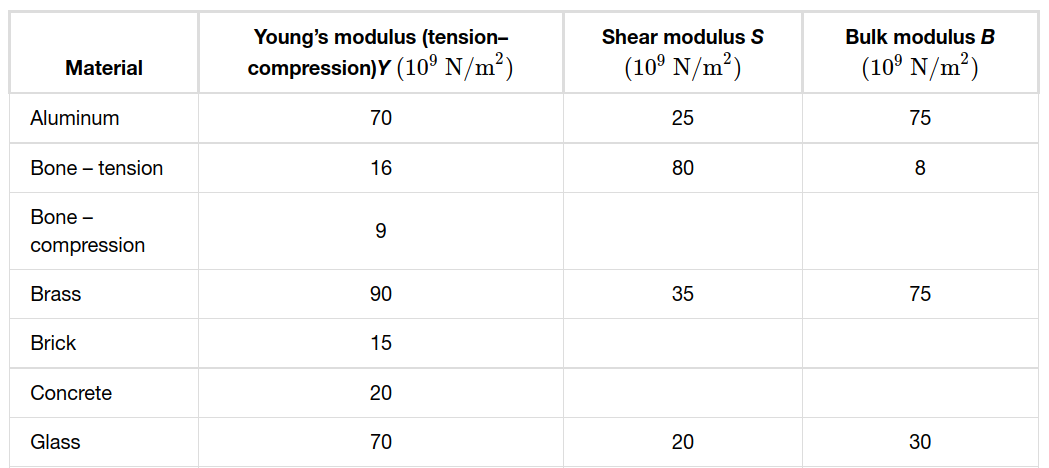
\includegraphics[width=0.6\textwidth]{figures/modulus.png} \\
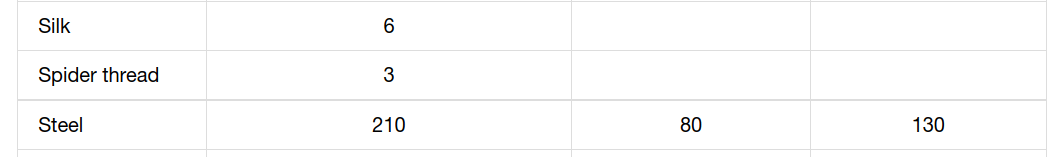
\includegraphics[width=0.6\textwidth]{figures/moduli2.png}
\caption{\label{fig:strain} (Left) A table of Young's moduli, shear moduli, and bulk moduli. (Right) A diagram of stress and strain on a rod of cross-sectional area $A$ and original length $L_0$.}
\end{figure}
\section{Chapter 5 - Stress and Strain}
\begin{enumerate}
\item Steel suspension cables are used to carry gondolas at ski resorts.  Find the Young's Modulus of steel in Figure 1.  Consider a suspension cable that (unstretched) has a length of 2 km. Calculate the $\Delta L$ in the steel cable, assuming that the cable has a diameter of 6 cm and the tension is $4.0 \times 10^6$ N. \\ \vspace{2cm}
\item What would the $\Delta L$ be if the original length was 3 km? (\textit{Hint: you can redo the problem with this new number, or just use scaling.}
\end{enumerate}

\end{document}
